\chapter[Soluciones individuales de series de Fourier]{Soluciones individuales de series de Fourier}
\label{cp:user-guide}

{
\parindent0pt

En este apartado se presentan las soluciones individuales de cada estudiante, desarrolladas a partir de las funciones propuestas por el profesor de la materia de Cómputo Paralelo.El objetivo principal de esta fase fue llevar a cabo el cálculo de la serie de Fourier correspondiente a cada función asignada, aplicando los métodos matemáticos adecuados para la obtención de los coeficientes y la expansión de la función en términos de senos y cosenos.
\vspace{10pt}

Cada integrante del equipo realizó los cálculos de manera independiente, asegurando un desarrollo detallado y estructurado de los coeficientes de Fourier. Para ello, se siguió el procedimiento estándar de integración para la obtención de los coeficientes \(a_0\), \(a_n\) y \(b_n\), que determinan la representación trigonométrica de la función en términos de series de Fourier.
\newpage
% \begin{verbatim}
% 00-Abstract.tex
% 01-Introduction.tex
% 02-User-Guide.tex
% ...
% \end{verbatim}
%---------------------------------------- Ilse

\section{Función resuelta por Castro Paez Ilse Yazbeth}
En este siguiente apartado, se presentan los cálculos para de la serie de Fourier de la función \(f(x)=9-3x-x^2\), correrpondientes a la figura \ref{fig:figure-ilse-01}, donde se muestran detalladamente el desarrollo hasta obtener el resultado. 

\begin{figure}[H]
    \centering
    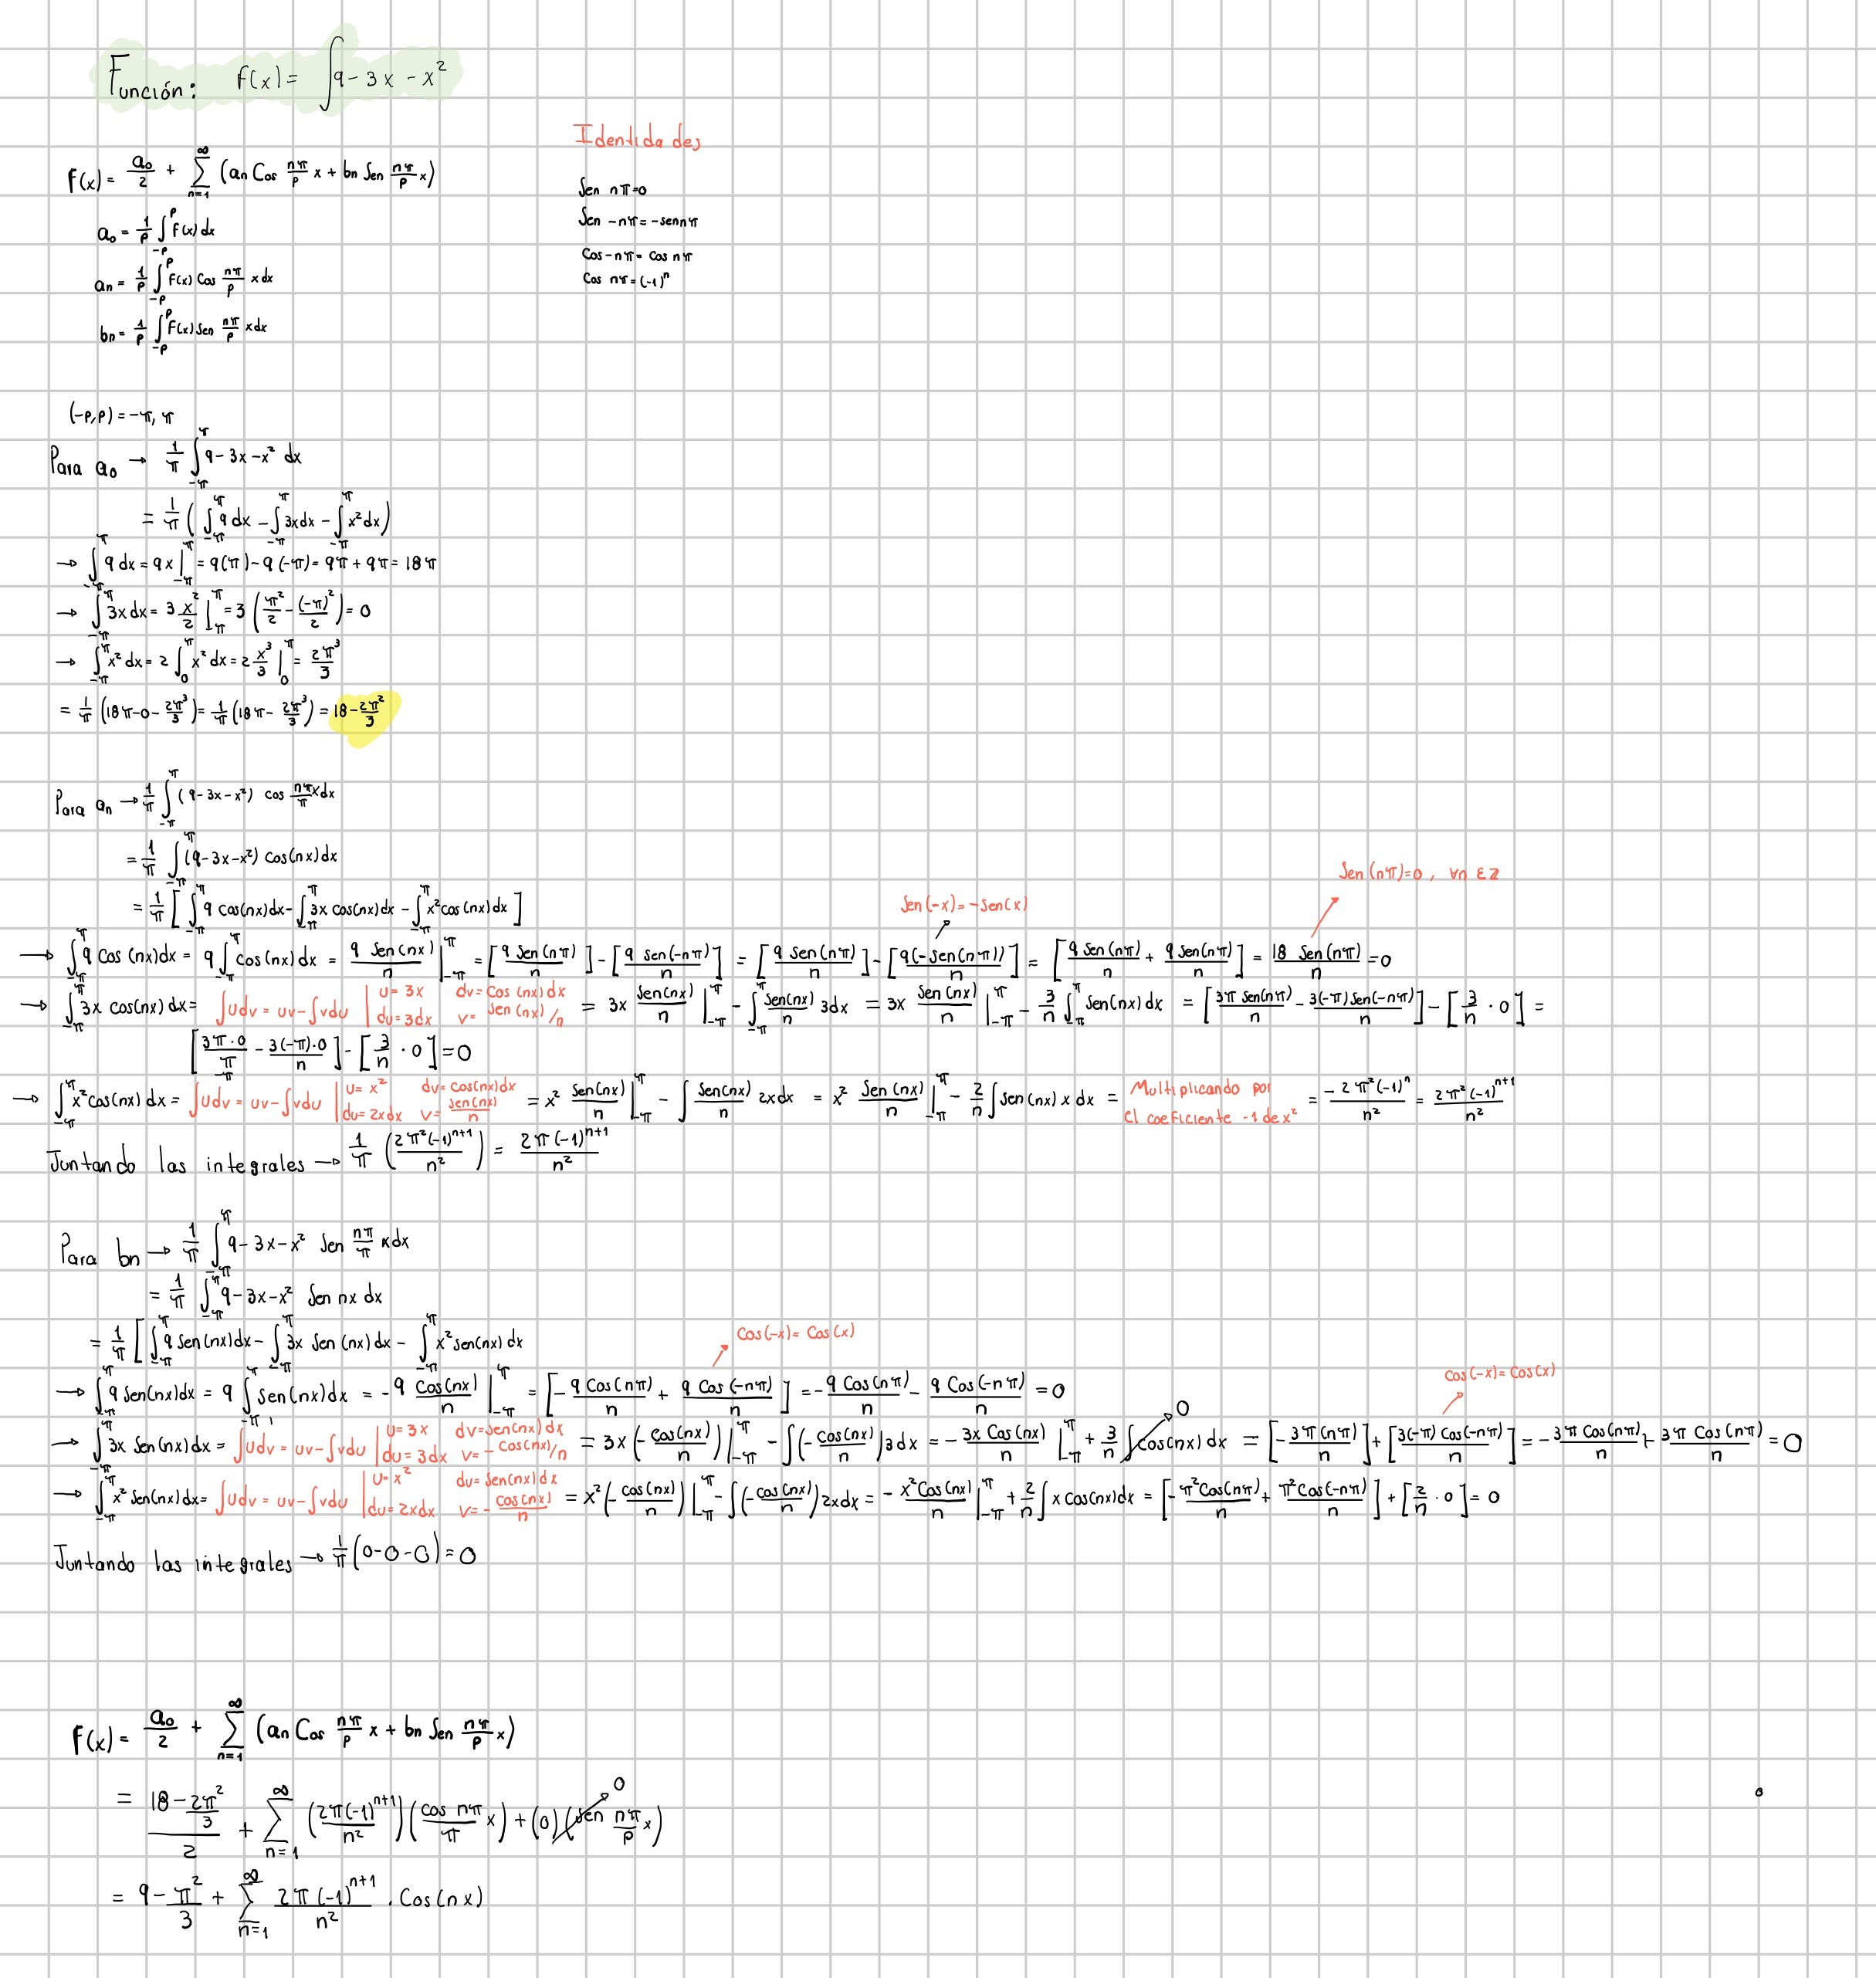
\includegraphics[width=\linewidth]{Figures/fourierIlse/fourierIlse.jpg}
    \caption[Cálculo de la función \(f(x)=9-3x-x^2\)]{Cálculo de la función \(f(x)=9-3x-x^2\), resuelto por Castro Paez Ilse Yazbeth}
    \label{fig:figure-ilse-01}
\end{figure}



%---------------------------------------- Daniel
\newpage
\section{Función resuelta por Catonga Tecla Daniel Isaí}
En el siguiente apartado, se presentan los cálculos para la obtención de los coeficientes de Fourier de la función asignada, \(f(x)=6-2x\), correspondientes a las figuras \ref{fig:figure-daniel-01} hasta \ref{fig:figure-daniel-04}. Se detallan las ecuaciones utilizadas y el procedimiento matemático seguido para su determinación.

\begin{figure}[H]
    \centering
    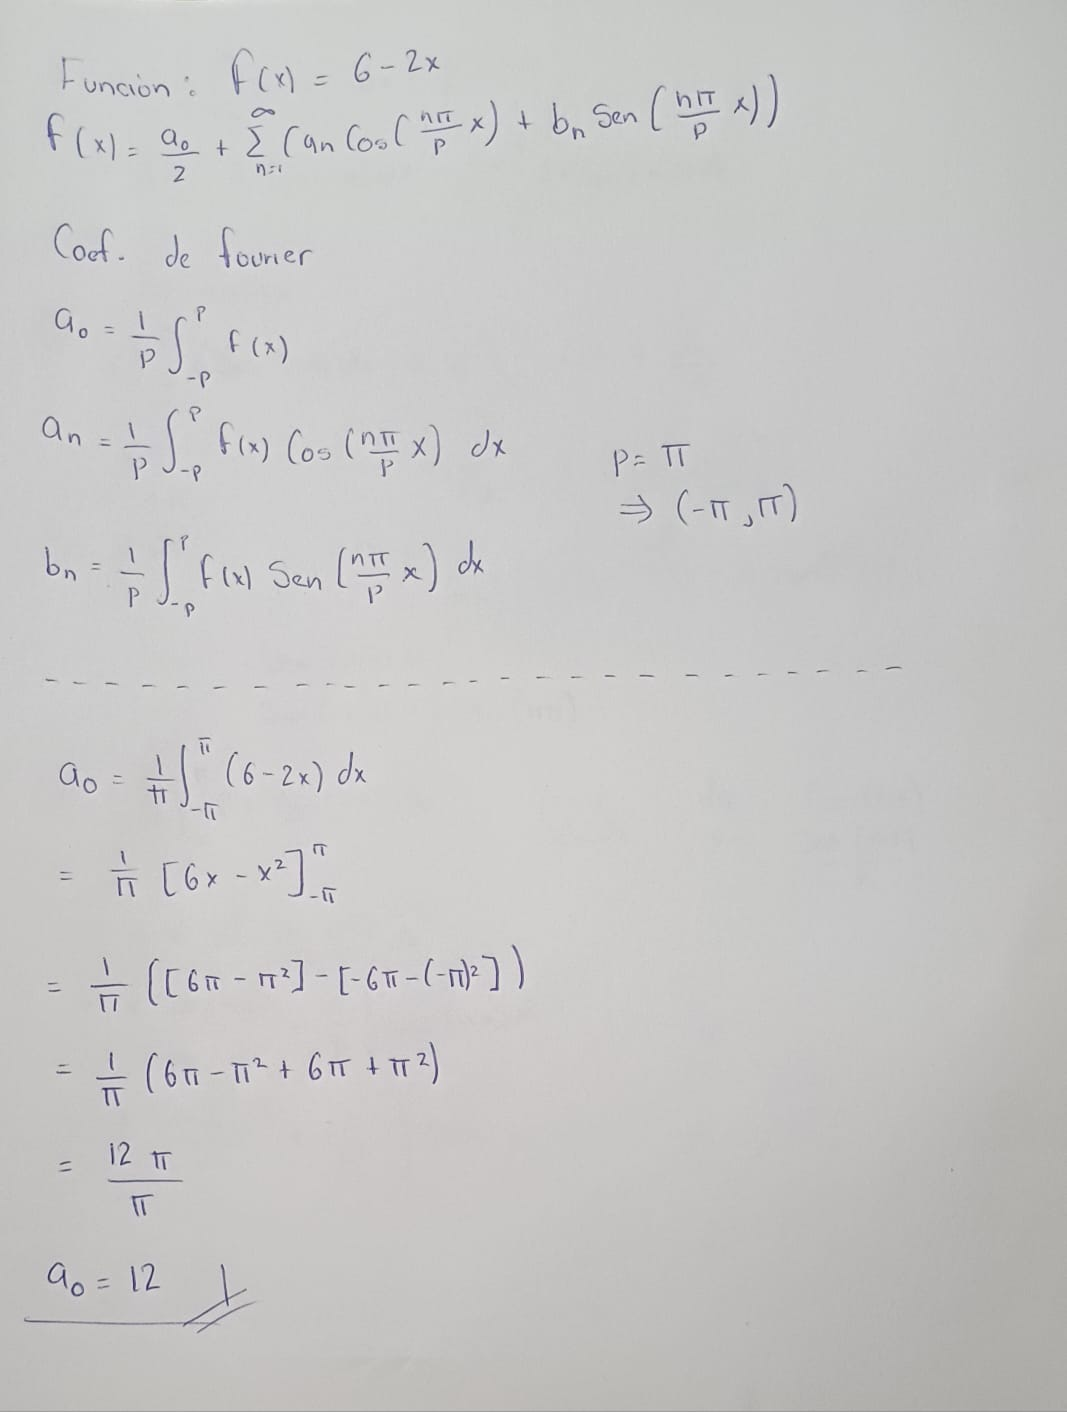
\includegraphics[width=\linewidth]{Figures/fourierDaniel/fourierDaniel1.jpg}
    \caption[Cálculo de \(a_0\) para \(f(x)=6-2x\)]{Cálculo de \(a_0\) para \(f(x)=6-2x\), resuelto por Catonga Tecla Daniel Isaí}
    \label{fig:figure-daniel-01}
\end{figure}

\begin{figure}[H]
    \centering
    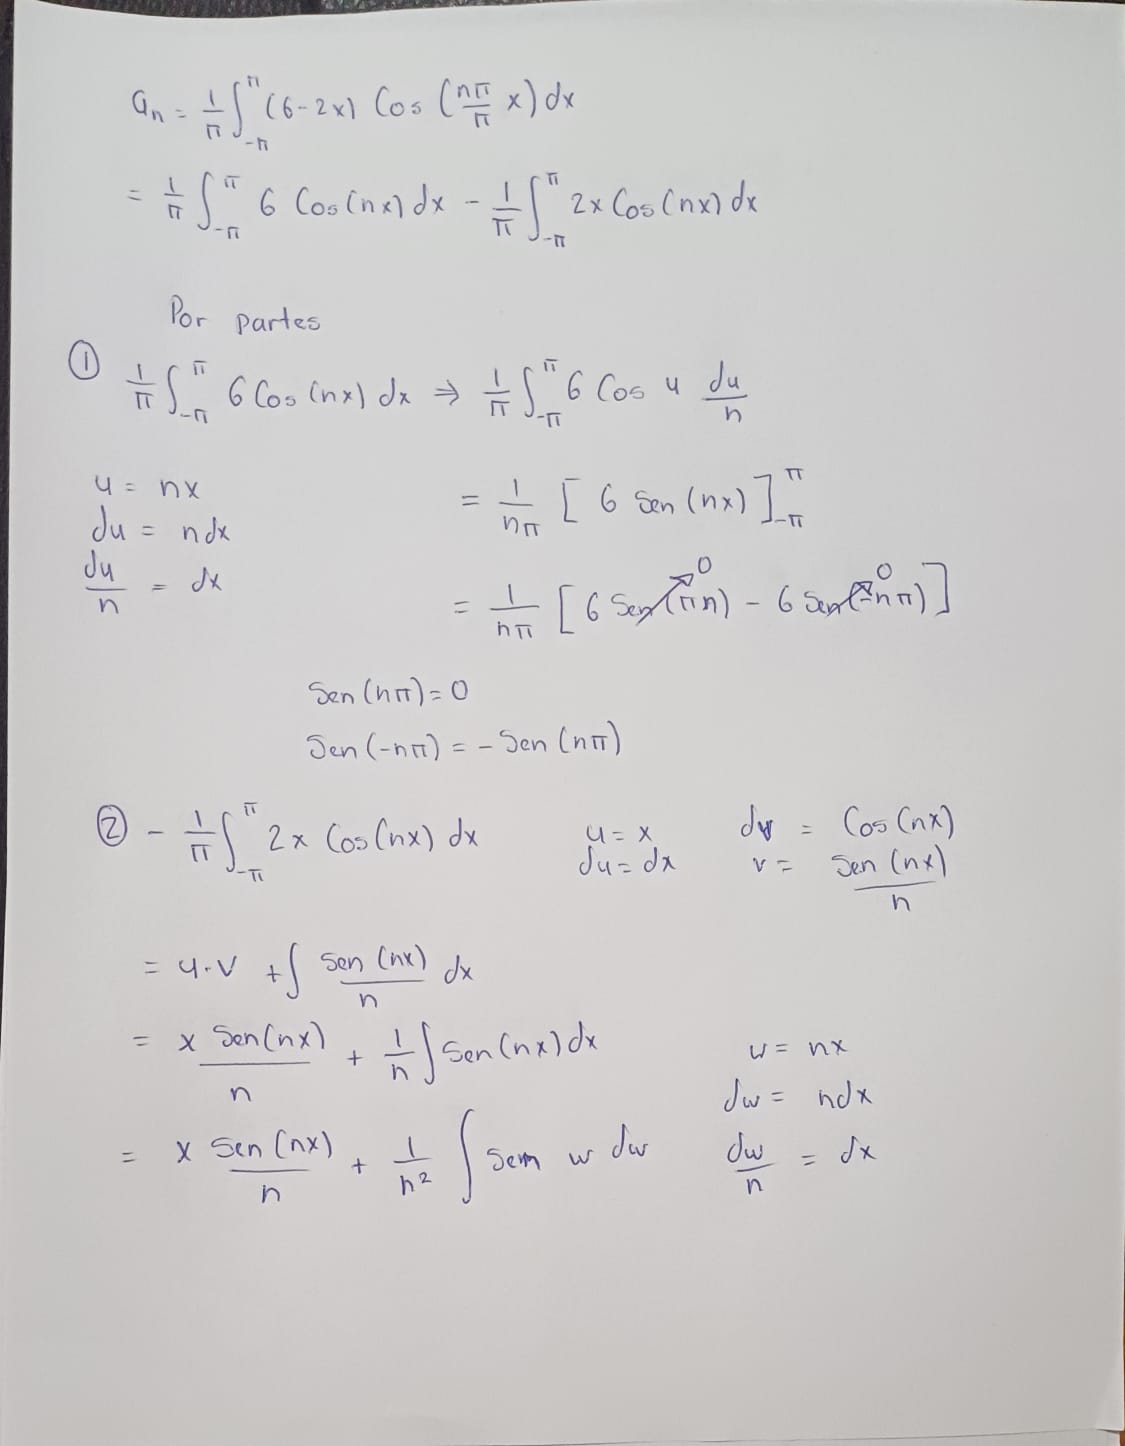
\includegraphics[width=\linewidth]{Figures/fourierDaniel/fourierDaniel2.jpg}
    \caption[Cálculo parcial de \(a_n\) para \(f(x) = 6 - 2x\)]{Desarrollo parcial del cálculo de los coeficientes \(a_n\) para la función \(f(x) = 6 - 2x\), resuelto por Catonga Tecla Daniel Isaí. El resultado final aún no se muestra.}
    \label{fig:figure-daniel-02}
\end{figure}

\begin{figure}[H]
    \centering
    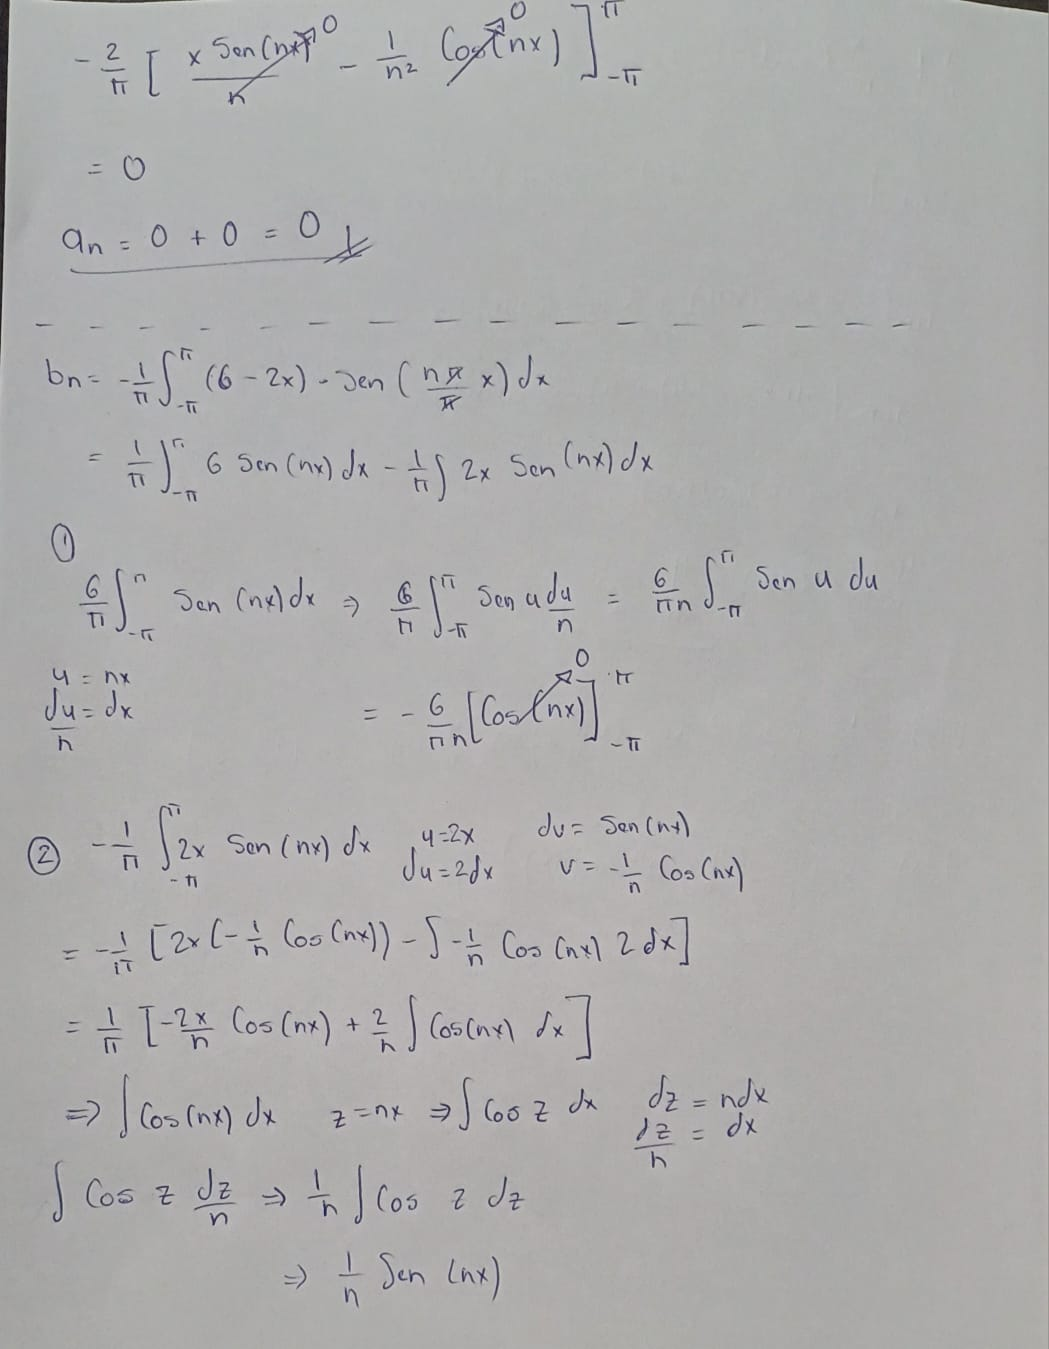
\includegraphics[width=\linewidth]{Figures/fourierDaniel/fourierDaniel3.jpg}
    \caption[Cálculo de \(a_n\) y desarrollo de \(b_n\) para \(f(x) = 6 - 2x\)]{Cálculo de \(a_n\) y desarrollo parcial de \(b_n\) para la función \(f(x) = 6 - 2x\), resuelto por Catonga Tecla Daniel Isaí.}
    \label{fig:figure-daniel-03}
\end{figure}

\begin{figure}[H]
    \centering
    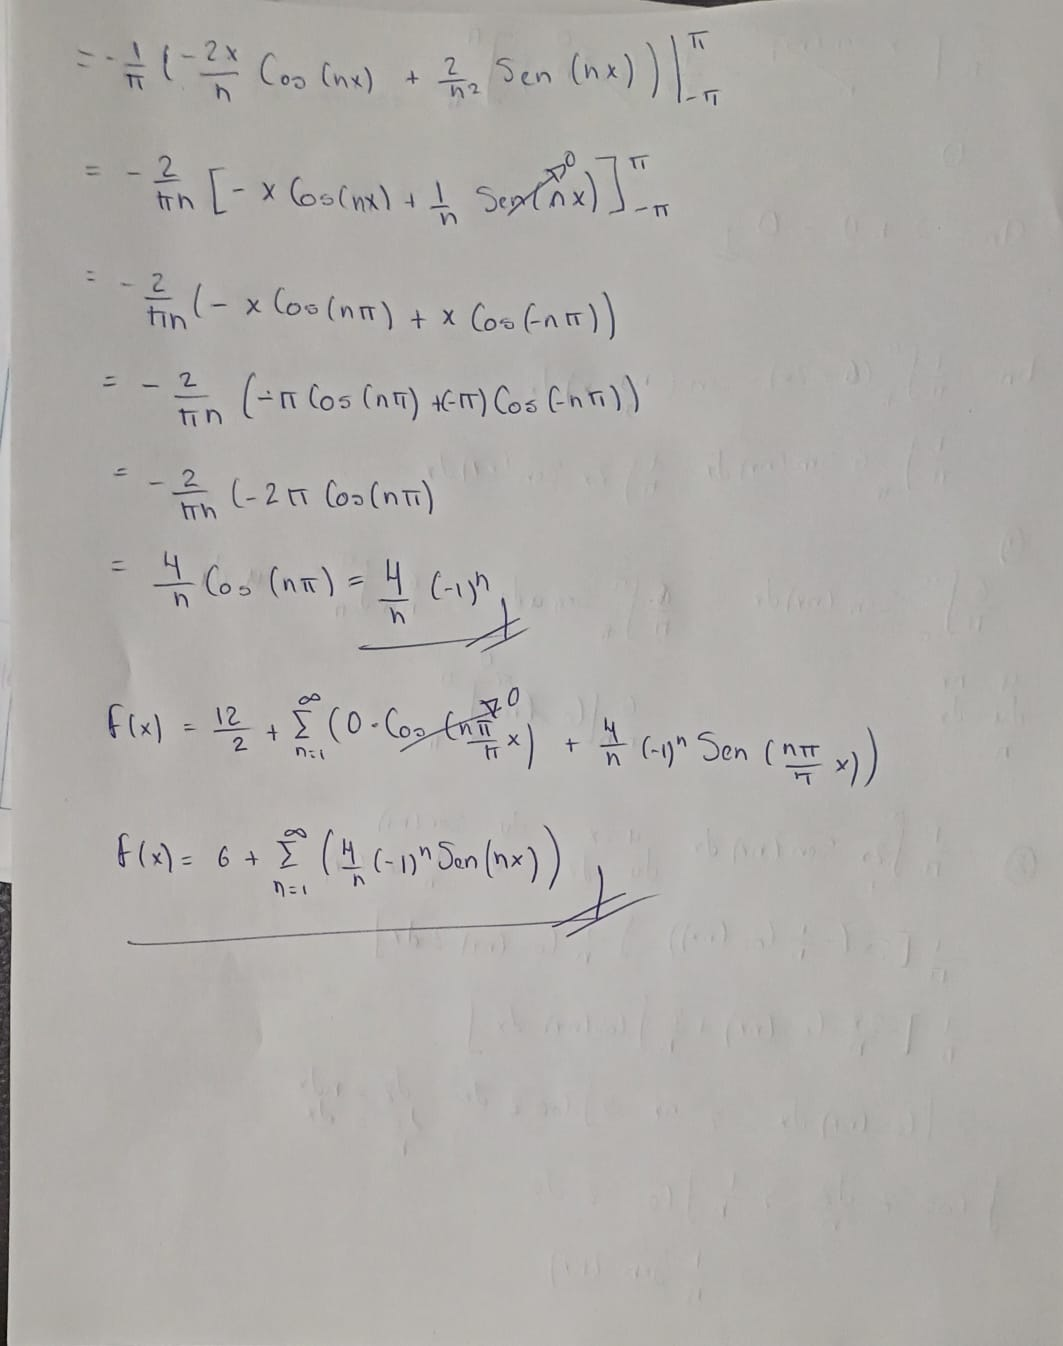
\includegraphics[width=\linewidth]{Figures/fourierDaniel/fourierDaniel4.jpg}
    \caption[Cálculo de \(b_n\) para \(f(x) = 6 - 2x\)]{Cálculo de \(b_n\) para la función \(f(x) = 6 - 2x\), mostrando la función reconstruida a partir de los coeficientes, resuelto por Catonga Tecla Daniel Isaí.}
    \label{fig:figure-daniel-04}
\end{figure}


%-------------------------------------------- Hariel
\newpage
\section{Función resuelta por Padilla Sanchez Hariel }
     En esta sección, se expone el procedimiento matemático para determinar los coeficientes de Fourier de la función \(f(x)=6-4x\). Se inicia con la ecuación general de la serie de Fourier y se procede al cálculo del coeficiente \(a_0\) como se muestra en la figura \ref{fig:figure-hariel-01},Para la obtención de \(a_n\), se emplea integración por partes, evidenciando la cancelación de ciertos términos. Se incluyen además observaciones sobre las propiedades trigonométricas utilizadas en el análisis.

%figura de a0 y an de Hariel 
    \begin{figure}[H]
        \centering
        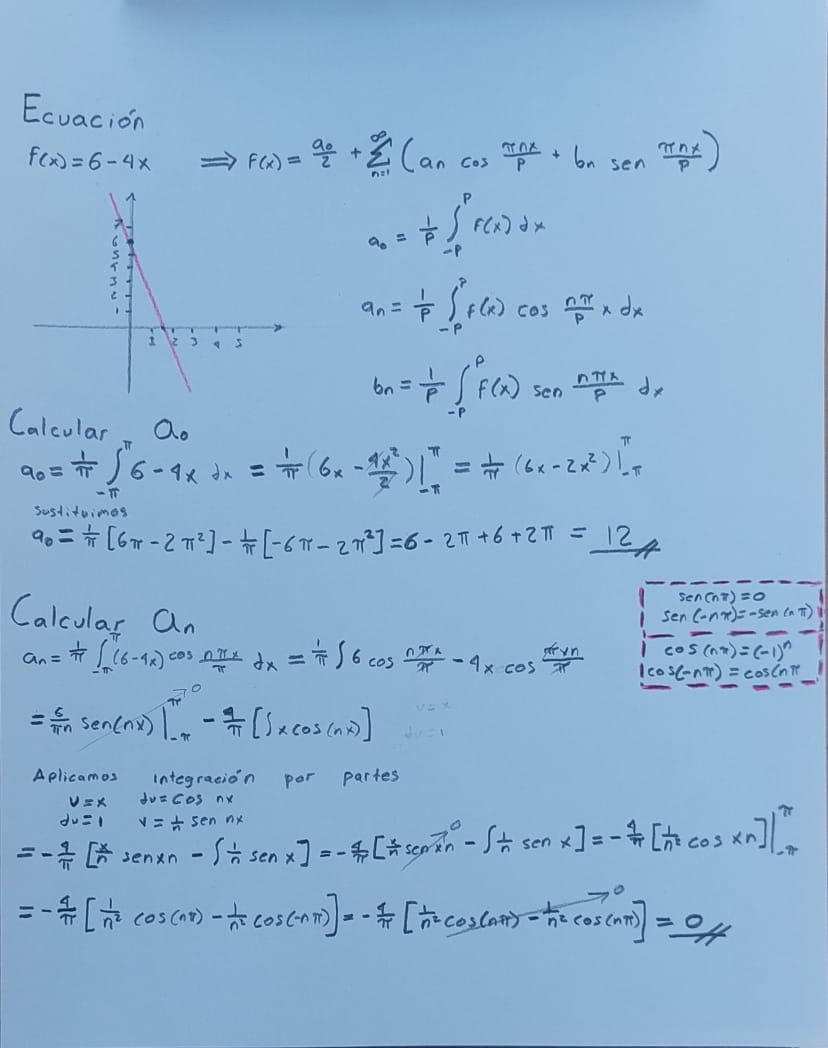
\includegraphics[width=\linewidth]{Figures/fourierHariel/fase1/funcion 1.jpg}
        \caption[Cálculo de \(a_0\) y \(a_n\) para \(f(x) = 6 - 4x\)]{Cálculo de \(a_0\) y \(a_n\) para la función \(f(x) = 6 - 4x\), resuelto por Padilla Sánchez Hariel.}
        \label{fig:figure-hariel-01}
    \end{figure}

    En el siguiente apartado, se presentan los cálculos para la obtención del coeficiente \(b_n\) de la serie de Fourier de la función \(f(x)=6-4x\). Se muestra el desarrollo de la integral correspondiente y la aplicación del método de integración por partes para resolver términos específicos como se muestra en la figura \ref{fig:figure-hariel-02}. Finalmente, se obtiene una expresión general para \(b_n\), la cual se utilizará en la reconstrucción de la función periódica.

%Figura de bn de Hariel
    \begin{figure}[H]
        \centering
        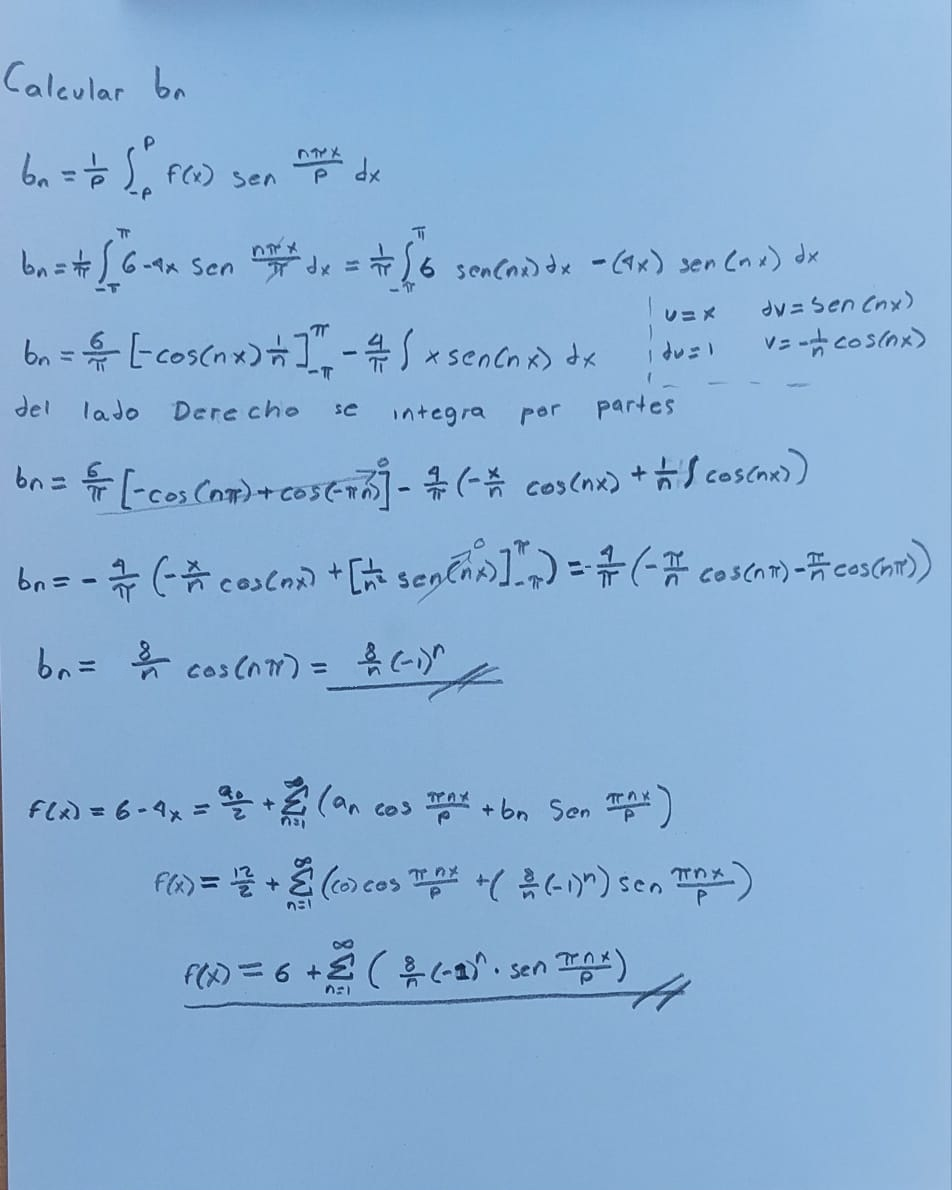
\includegraphics[width=\linewidth]{Figures/fourierHariel/fase1/funcion 2.jpg}
        \caption[Cálculo de \(b_n\) para \(f(x) = 6 - 4x\)]{Cálculo de \(b_n\) para la función \(f(x) = 6 - 4x\), resuelto por Padilla Sánchez Hariel.}
        \label{fig:figure-hariel-02}
    \end{figure}

%-------------------------------------------- Manuel
\section{Función resuelta por Olguin Castillo Víctor Manuel }
    A continuacion se calculan los coeficientes de Fourier asociados a la función \(f(x)=x^2-3x-3\) . 

%figura de a0
    \begin{figure}[H]
        \centering
        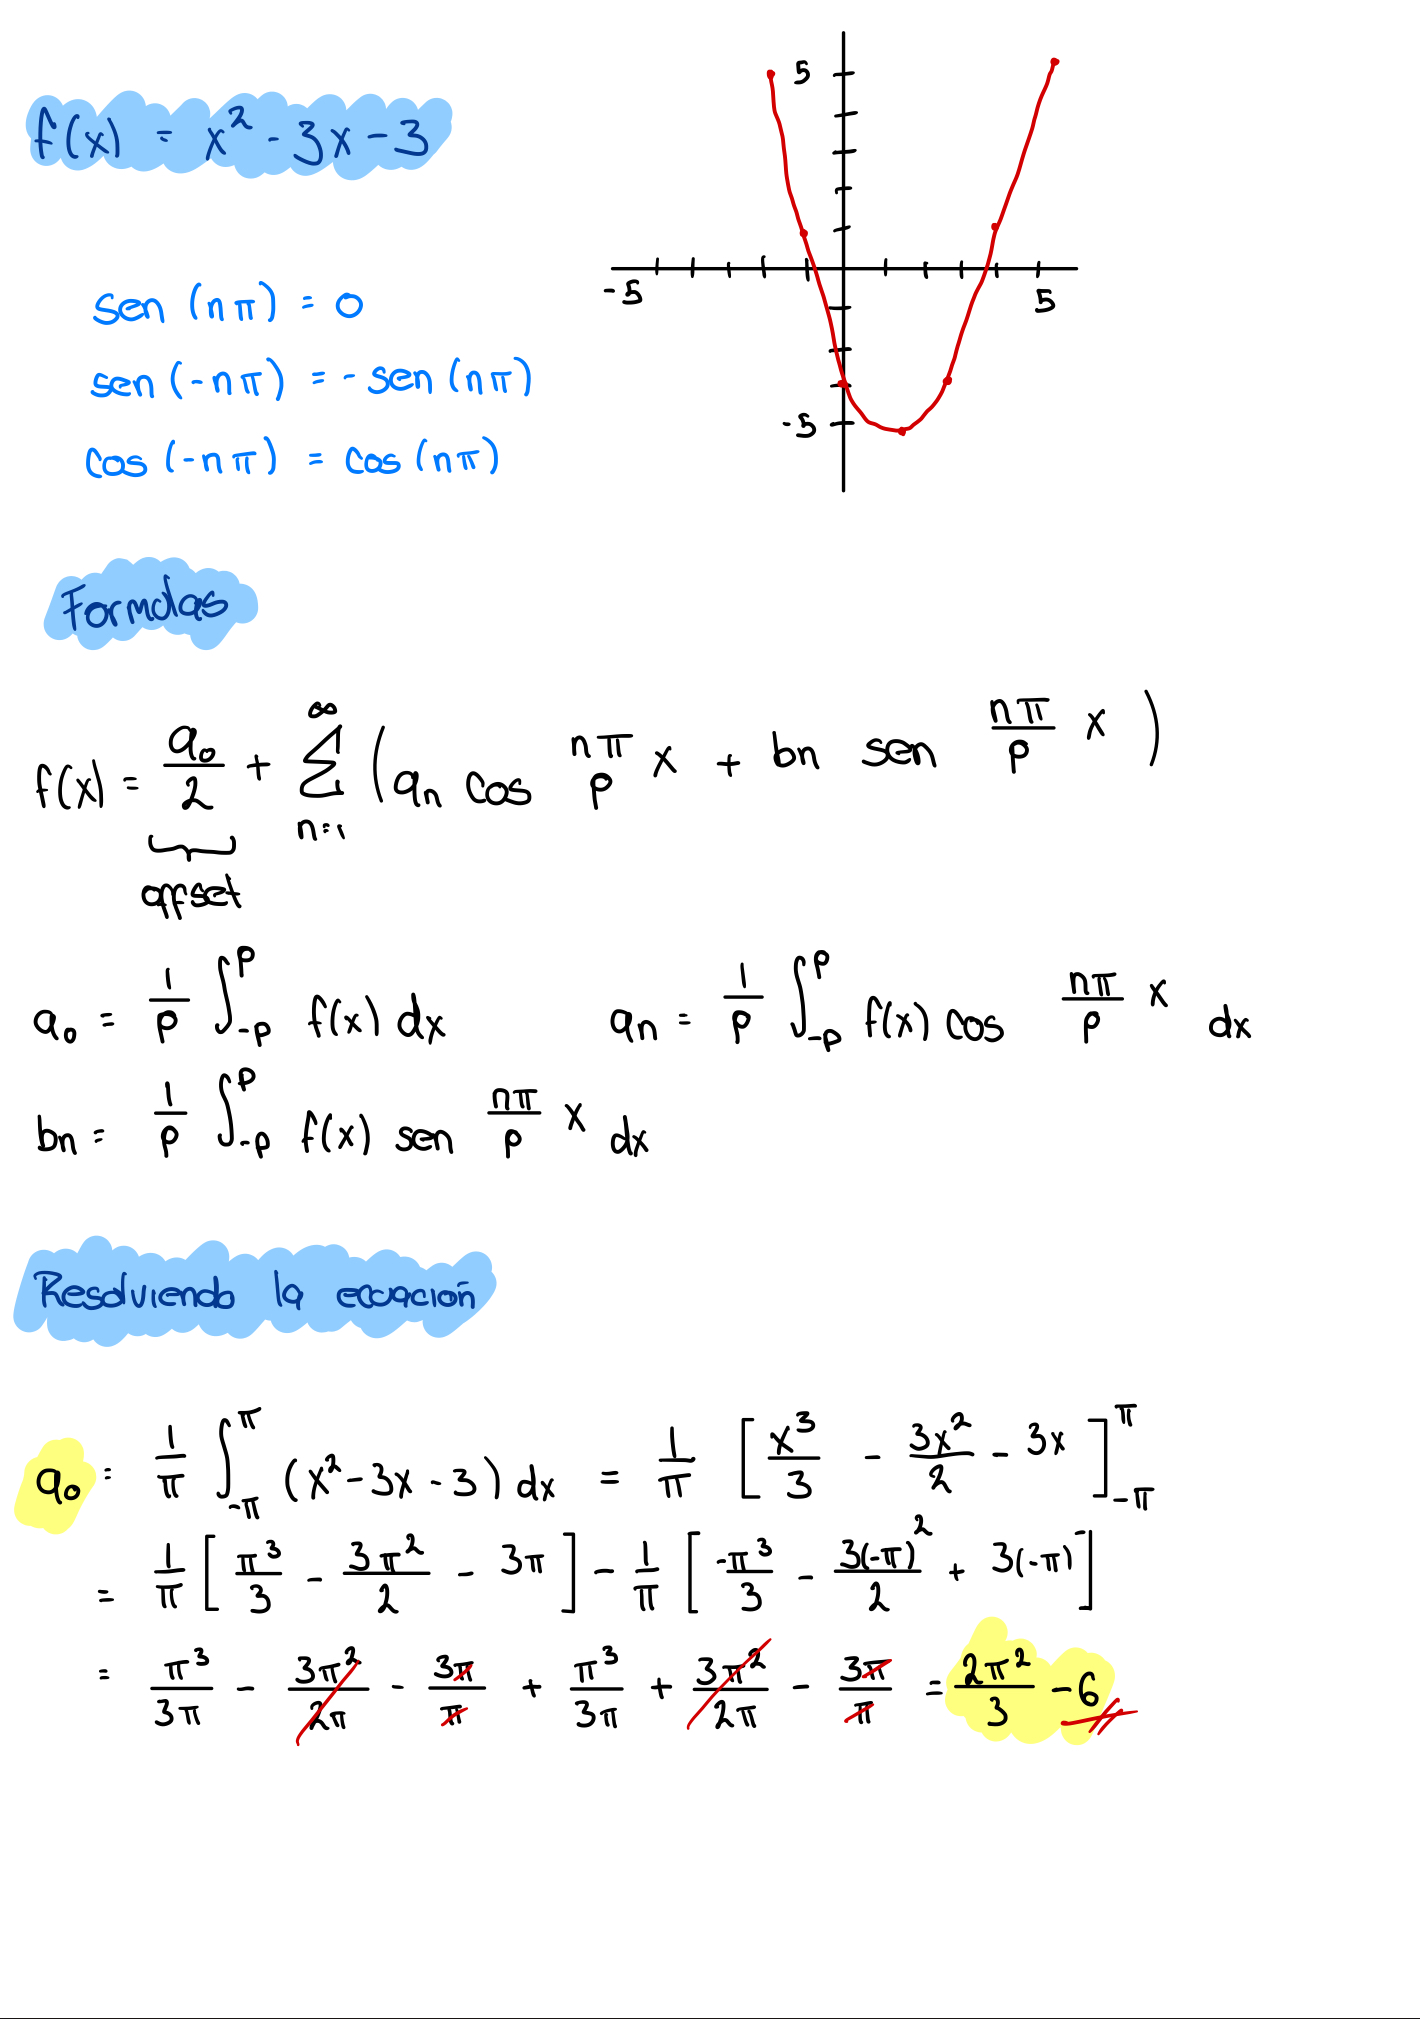
\includegraphics[width=\linewidth]{Figures/fourierManuel/a0.jpeg}
        \caption[Cálculo de \(a_0\)]{Cálculo de \(a_0\), resuelto por Olguin Castillo.}
        \label{fig:figure-manuel-01}
    \end{figure}

%figura de a0
    \begin{figure}[H]
        \centering
        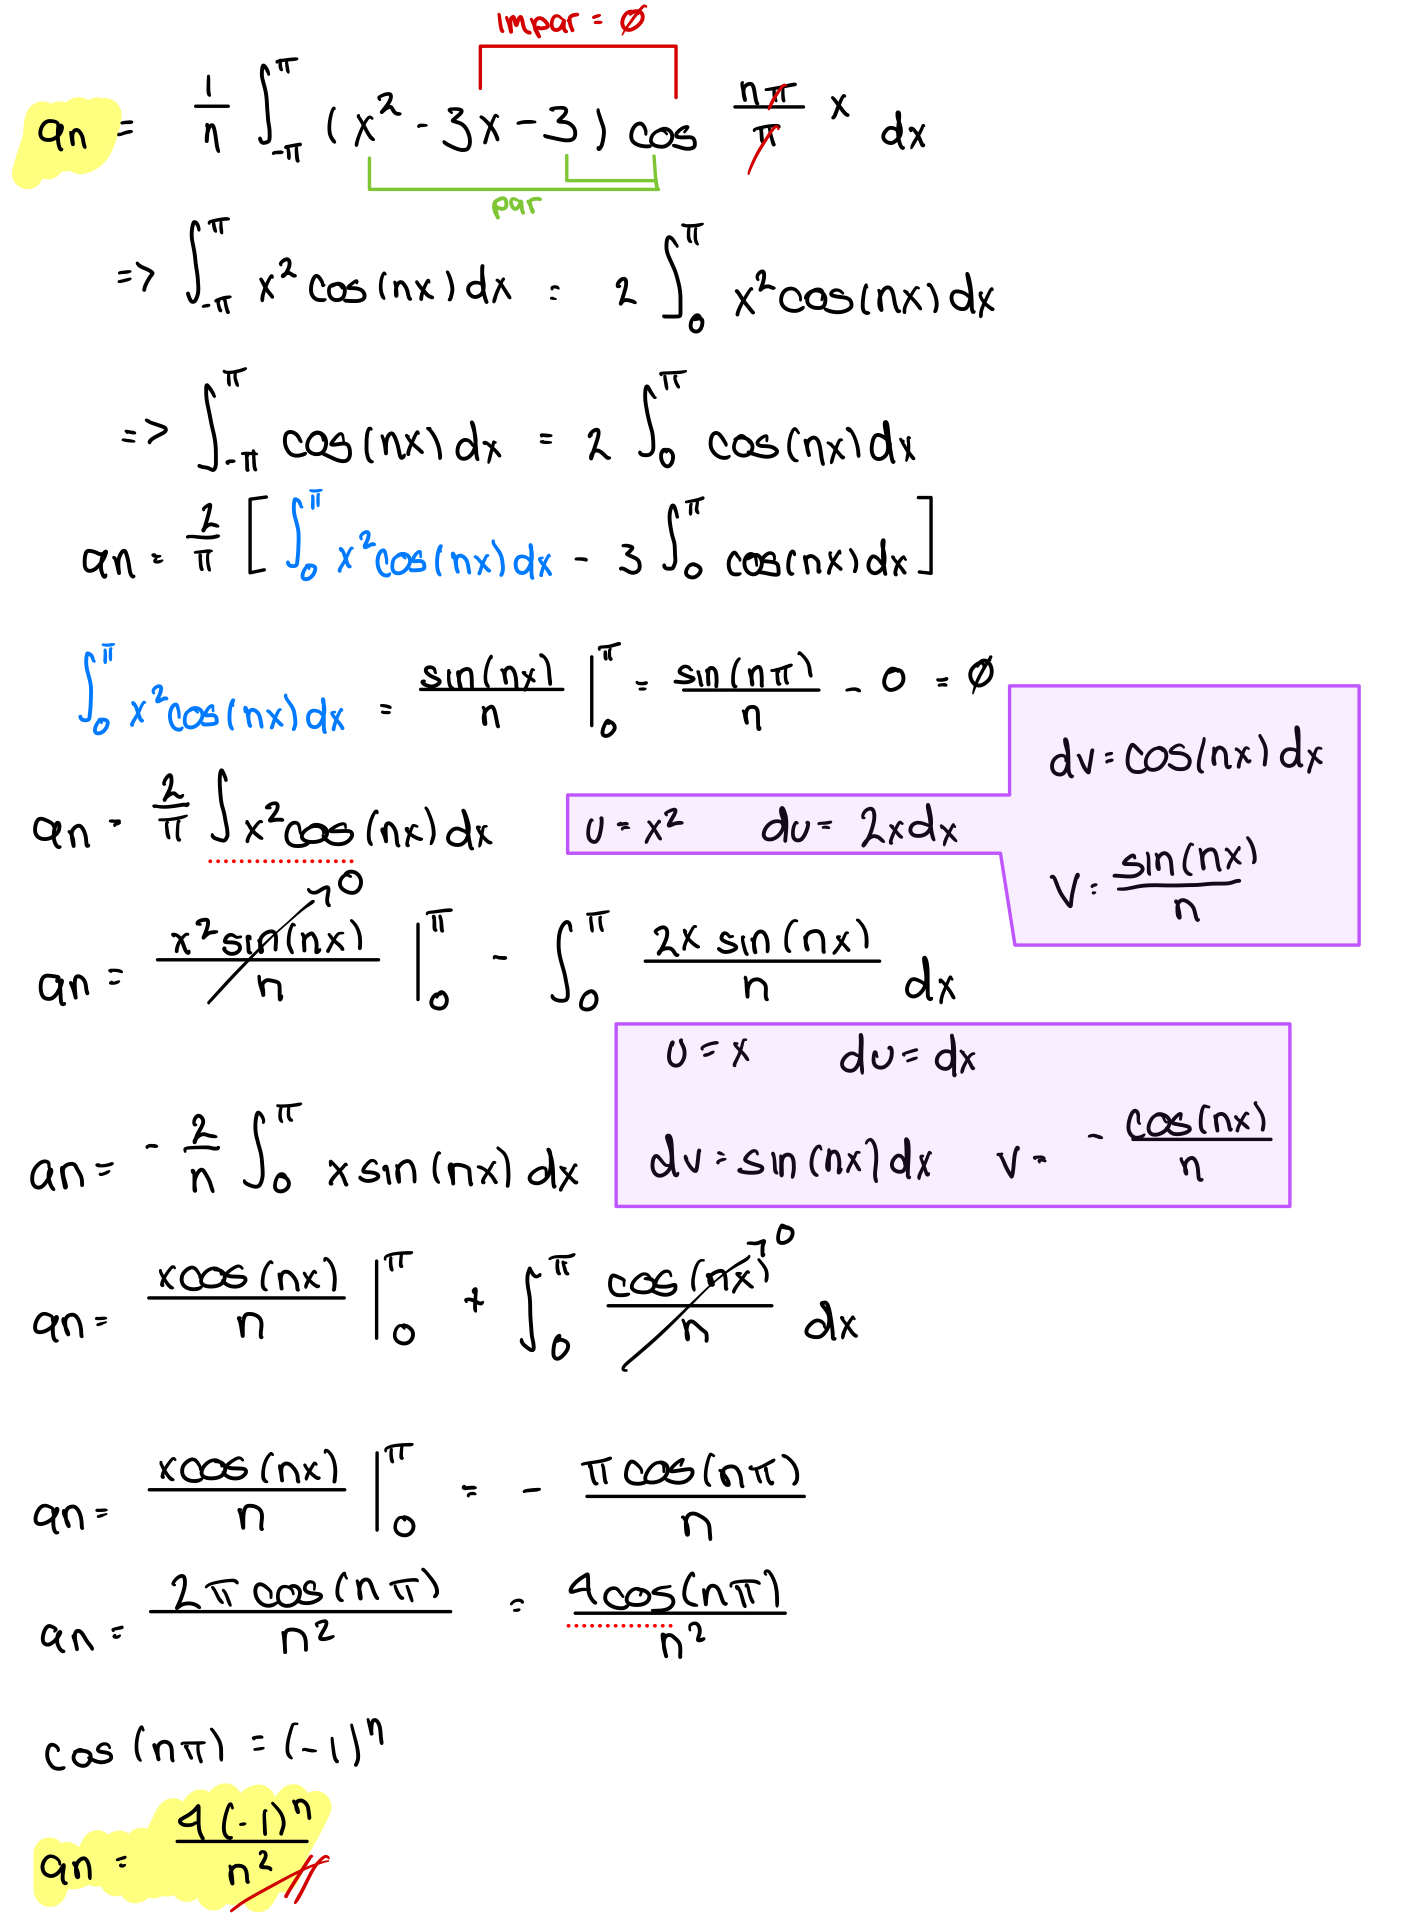
\includegraphics[width=\linewidth]{Figures/fourierManuel/an.jpeg}
        \caption[Cálculo de \(a_n\)]{Cálculo de \(a_n\), resuelto por Olguin Castillo.}
        \label{fig:figure-manuel-02}
    \end{figure}

\begin{figure}[H]
        \centering
        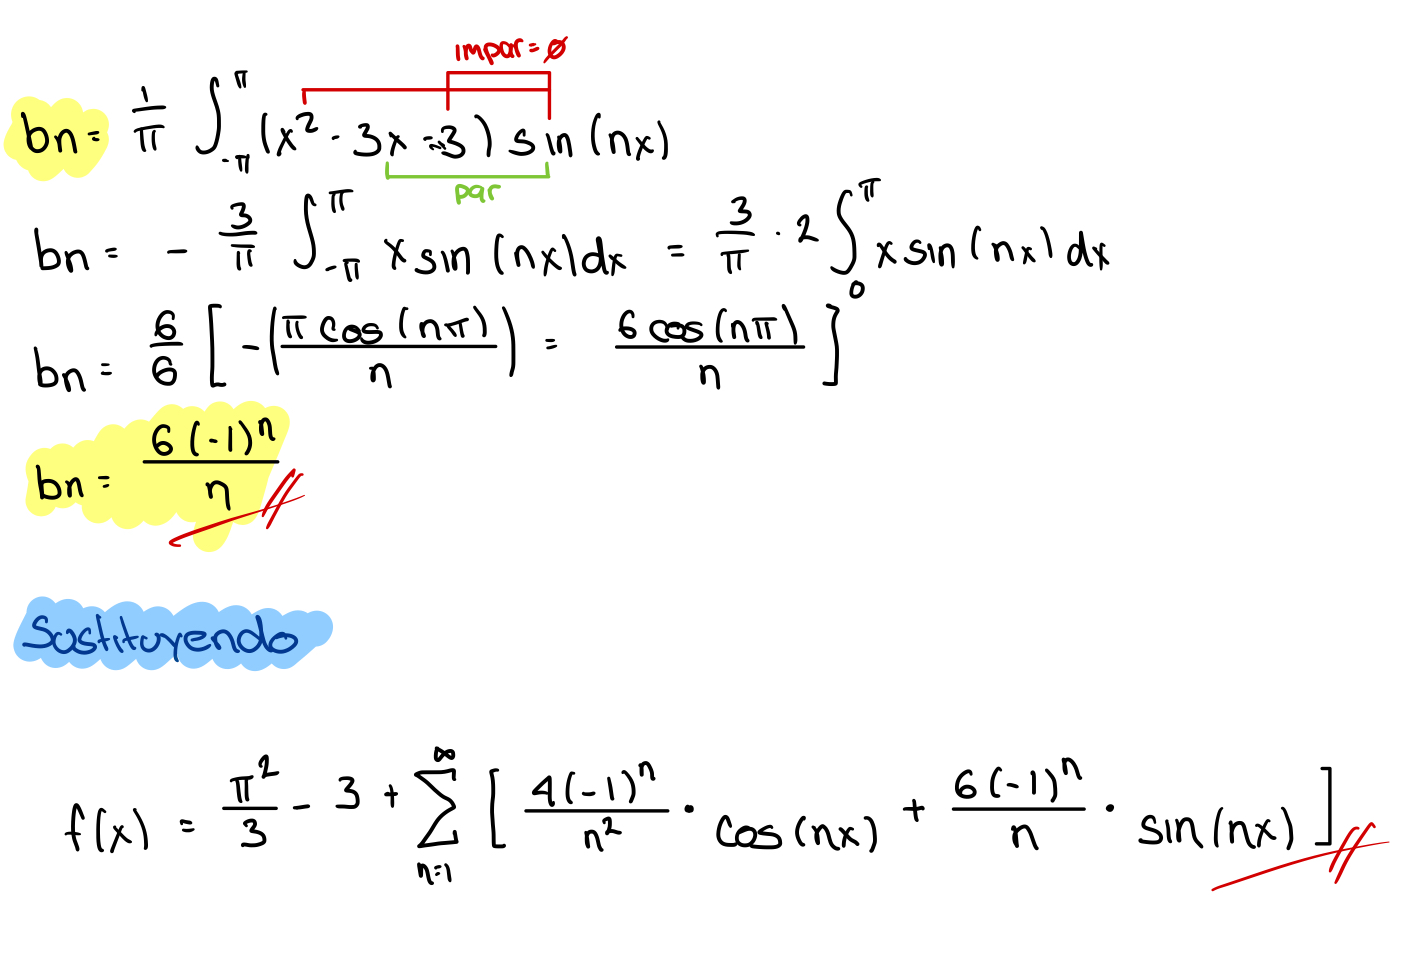
\includegraphics[width=\linewidth]{Figures/fourierManuel/bn.jpeg}
        \caption[Cálculo de \(b_n\)]{Cálculo de \(b_n\), resuelto por Olguin Castillo.}
        \label{fig:figure-manuel-03}
    \end{figure}

El método se basa en la expansión en series de Fourie usando simplificaciones algebraicas y las propiedades trigonométricas que permiten reducir la expresión final.



%-------------------------------------------- Fase 3
\section{Programa en C para el cálculo de la serie de Fourier}
    El objetivo del programa es calcular una aproximación de la serie de Fourier para la función \(f(x)=6−4x\) ., utilizando un enfoque paralelo basado en la creación de procesos hijos, memoria compartida y semáforos en el sistema operativo Linux. Esta función es impar, por lo tanto, su serie de Fourier se puede expresar únicamente con términos en seno, en la forma:
\[
f(x) \approx a_0 + \sum_{n=1}^{N} b_n \sin(nx)
\]

donde \( a_0 = 6 \) y los coeficientes \( b_n \) están dados por:

\[
b_n = \frac{8}{n}(-1)^n
\]

Para este programa, se consideran valores de \( x \) desde -3.14 hasta 3.14 con un incremento de 0.15. Se calculan los primeros 10 términos de la serie de Fourier, y cada uno de estos es calculado por un proceso hijo independiente. Los resultados son almacenados en una matriz en memoria compartida, protegida por un semáforo para evitar conflictos en la escritura concurrente. Finalmente, se suman todos los términos y se genera un archivo CSV con los resultados.


Para la implementación en C se hace uso de varias bibliotecas. La biblioteca \texttt{stdio.h} se emplea para las operaciones de entrada y salida estándar como la lectura y escritura en archivos. La biblioteca \texttt{stdlib.h} se utiliza para funciones de control como \texttt{exit()} y la gestión de memoria dinámica. \texttt{unistd.h} proporciona el uso de \texttt{fork()}, fundamental para la creación de procesos hijos. Además, se incluyen \texttt{sys/ipc.h}, \texttt{sys/shm.h} y \texttt{sys/sem.h}, necesarias para trabajar con memoria compartida y semáforos bajo el esquema de IPC System V en Linux. Finalmente, \texttt{math.h} permite el uso de funciones matemáticas como \texttt{sin()} y \texttt{pow()}.

\begin{figure}[H]
    \centering
    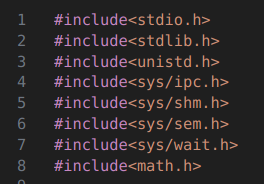
\includegraphics[width=0.8\linewidth]{Figures/codigo/librerias.png}
    \caption[Librerías utilizadas en el programa]{Fragmento de código que muestra las librerías utilizadas en el programa.}
    \label{fig:codigo-funcion}
\end{figure}


La función \texttt{funcion} tiene la responsabilidad de calcular cada término individual de la serie de Fourier. Recibe como parámetros el valor de \( n \) y el punto \( x \), y devuelve el resultado de la expresión \( \frac{8}{n} (-1)^n \sin(nx) \), que corresponde al coeficiente \( b_n \sin(nx) \). Este valor es calculado por cada proceso hijo para los diferentes valores de \( x \).

\begin{figure}[H]
    \centering
    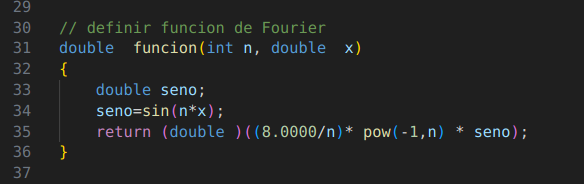
\includegraphics[width=0.8\linewidth]{Figures/codigo/funcion.png}
    \caption[Función para calcular \(b_n \sin(nx)\)]{Fragmento de código de la función que calcula el término \(b_n \sin(nx)\).}
    \label{fig:codigo-funcion}
\end{figure}

Para controlar el acceso concurrente a la memoria compartida, se definen dos funciones auxiliares: \texttt{down} y \texttt{up}. La función \texttt{down} realiza una operación de espera o bloqueo, decrementando el valor del semáforo. Esto indica que un proceso ha ingresado a la sección crítica. Por otro lado, la función \texttt{up} incrementa el semáforo, liberando así la sección crítica para que otro proceso pueda acceder. Estas funciones garantizan la exclusión mutua al momento de escribir en la memoria compartida.

La función \texttt{Crea\_semaforo} encapsula el proceso de creación de un semáforo. Se basa en una clave generada por la función \texttt{ftok()} y lo crea con permisos de lectura y escritura para todos los usuarios. Se inicializa con un valor de 1, lo cual significa que inicialmente la sección crítica está libre.

\begin{figure}[H]
    \centering
    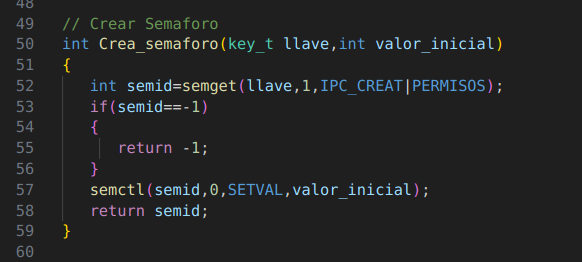
\includegraphics[width=0.9\linewidth]{Figures/codigo/semaforo.png}
    \caption[Creación del semáforo]{Fragmento de código que muestra la creación del semáforo.}
    \label{fig:semaforo}
\end{figure}

La función \texttt{crearArchivo} se utiliza para crear archivos vacíos que posteriormente son usados por \texttt{ftok()} para generar claves únicas. Aunque no escriben información dentro del archivo, su existencia es necesaria para que \texttt{ftok()} funcione correctamente. Se crean archivos para la memoria compartida y el semáforo.

\begin{figure}[H]
    \centering
    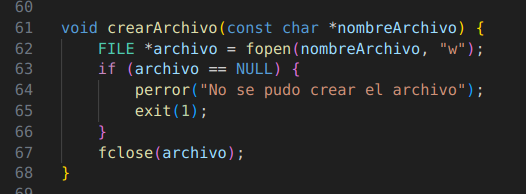
\includegraphics[width=0.9\linewidth]{Figures/codigo/crearArchivo.png}
    \caption[Creación de archivos vacíos]{Fragmento de código que muestra la creación de archivos vacíos para la generación de claves.}
    \label{fig:archivo_crear}
\end{figure}

Dentro de la función \texttt{main}, se calcula primero la cantidad de puntos de evaluación entre los valores de -3.14 y 3.14, considerando un incremento de 0.15. Esta cantidad determina el tamaño del arreglo de valores de \( x \), así como el tamaño de la memoria compartida necesaria para guardar todos los resultados. Luego, se generan las claves para la memoria y el semáforo, y se crean ambos recursos. A continuación, se calcula el arreglo de valores de \( x \) y se almacena en un arreglo auxiliar.

\begin{figure}[H]
    \centering
    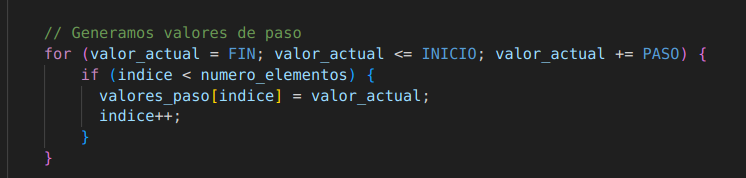
\includegraphics[width=0.9\linewidth]{Figures/codigo/x_values.png}
    \caption[Generación de valores de \(x\)]{Cálculo de los valores de \(x\) que se usarán en la evaluación de los términos de la serie.}
    \label{fig:x-values}
\end{figure}

Posteriormente, se crea el primer proceso hijo que escribe directamente la constante \( a_0 = 6 \) en toda la primera fila de la matriz compartida. Después, se crean otros diez procesos hijos. Cada uno de estos se encarga de calcular los valores del término \( b_n \sin(nx) \) para cada valor de \( x \). Para evitar que múltiples procesos escriban al mismo tiempo, cada proceso llama a \texttt{down} antes de escribir y a \texttt{up} después de terminar de escribir.

\begin{figure}[H]
    \centering
    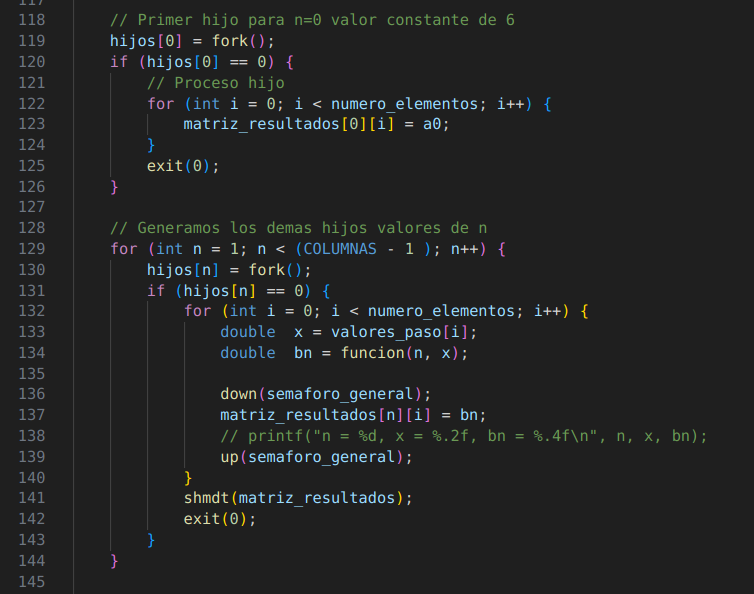
\includegraphics[width=0.9\linewidth]{Figures/codigo/procesos_hijos.png}
    \caption[Creación y sincronización de procesos]{Código que muestra la creación de procesos hijos y el uso de semáforo para escritura sincronizada.}
    \label{fig:procesos-hijos}
\end{figure}


El proceso padre se encarga de esperar a que todos los procesos hijos terminen su ejecución. Para ello, utiliza múltiples llamadas a la función \texttt{wait()}. Una vez que todos los hijos han terminado, el padre realiza la suma de todos los términos calculados para cada valor de \( x \). Esta suma se almacena en la última fila de la matriz compartida.

\begin{figure}[H]
    \centering
    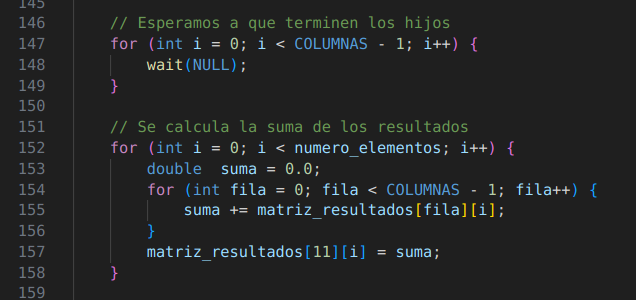
\includegraphics[width=0.9\linewidth]{Figures/codigo/suma_resultados.png}
    \caption[Suma de los resultados y generación de archivo]{Código que suma los términos de la serie para cada valor de \( x \) y escribe los resultados en un archivo.}
    \label{fig:suma-resultados}
\end{figure}

Finalmente, se abre un archivo CSV llamado \texttt{resultados.csv} y se imprimen en él todos los resultados, incluyendo el valor de \( x \), cada término de la serie y la suma total.

\begin{figure}[H]
    \centering
    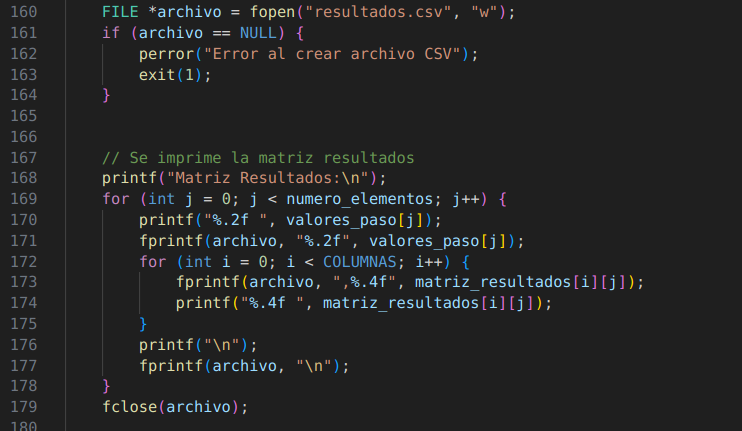
\includegraphics[width=0.9\linewidth]{Figures/codigo/escritura_archivo.png}
    \caption[Escritura de resultados en archivo CSV]{Código que muestra la escritura de los resultados en un archivo CSV.}
    \label{fig:escritura-archivo}
\end{figure}


Al finalizar la ejecución del programa, se imprime en la consola la matriz completa de resultados. En cada línea se muestra un valor de \(x\), seguido por los términos \(a_0\) y \(b_n \sin(nx)\) calculados por cada proceso hijo para ese punto, así como la suma total de todos los términos, que representa la aproximación de \(f(x)\) mediante la serie de Fourier. Esta visualización permite al usuario verificar que los cálculos se han realizado correctamente y apreciar el comportamiento de la aproximación en el dominio especificado.

\begin{figure}[H]
    \centering
    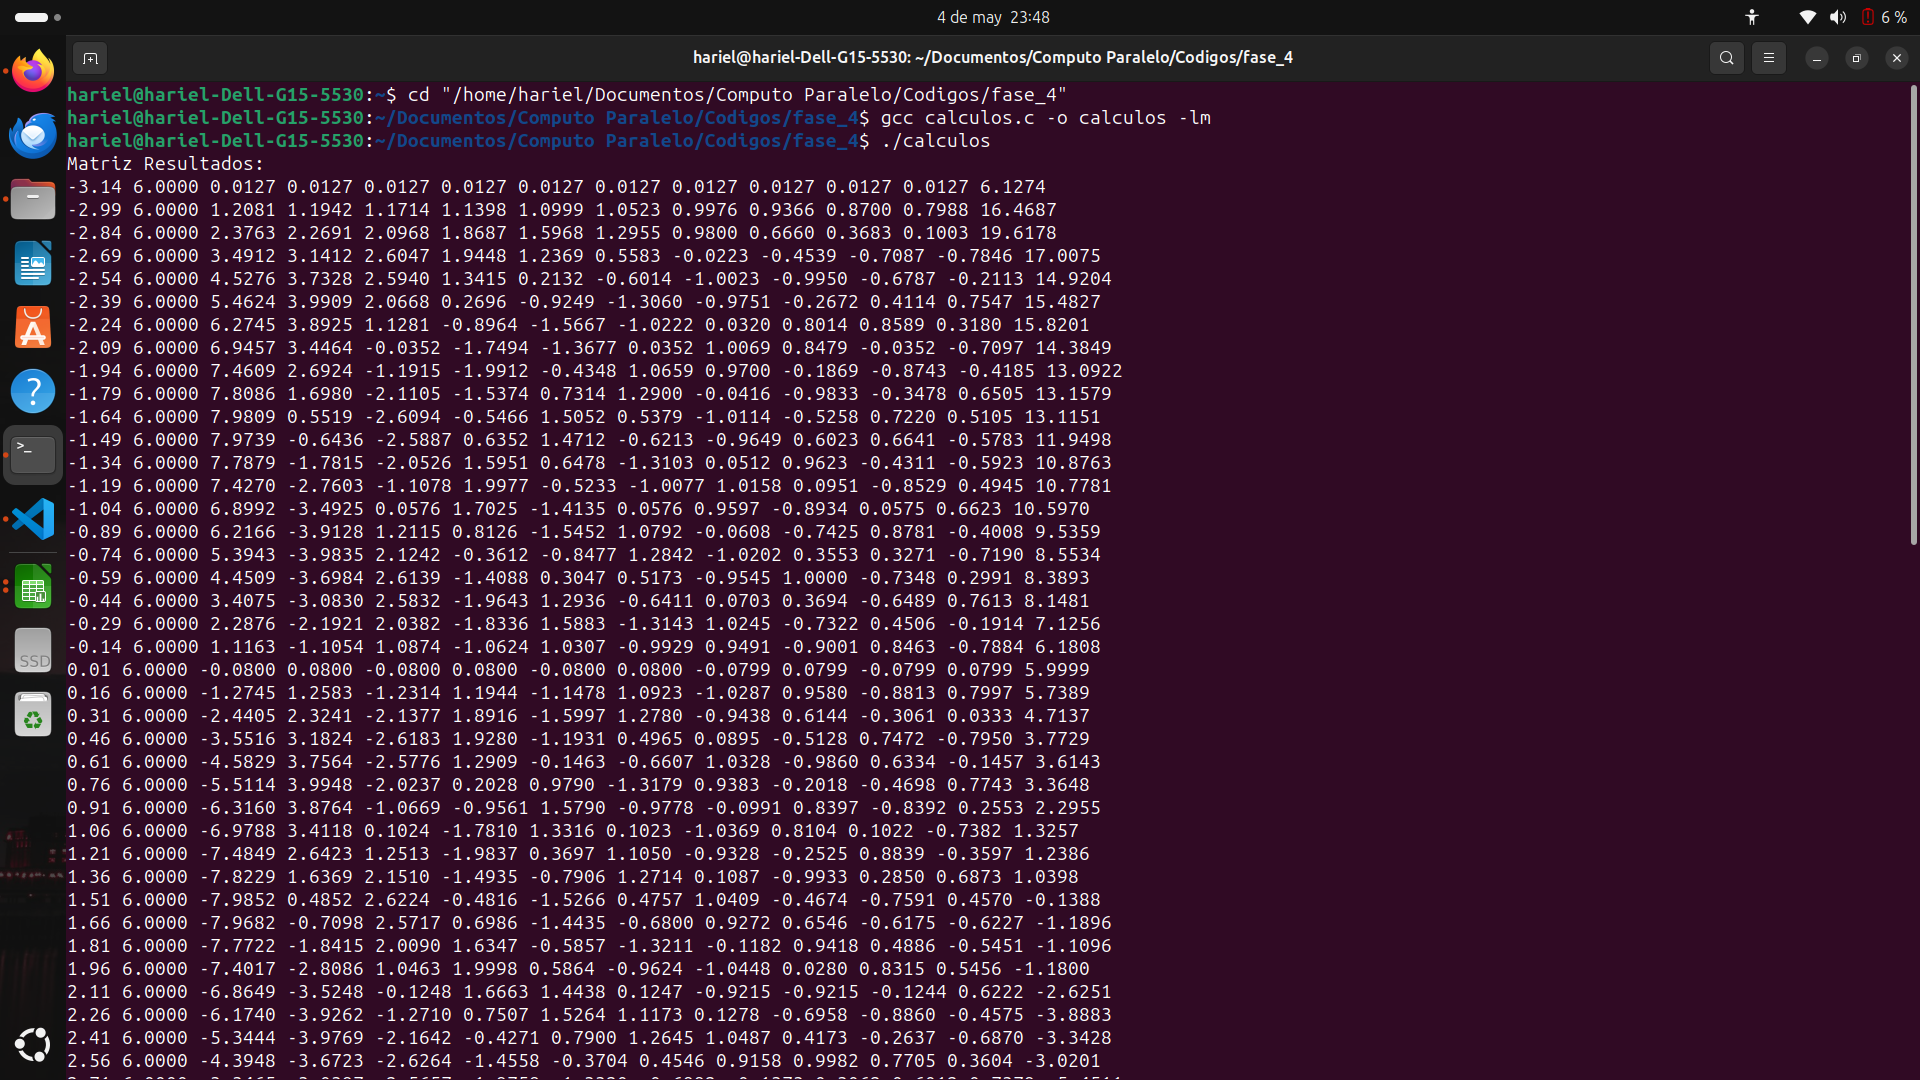
\includegraphics[width=0.9\linewidth]{Figures/codigo/impresion_matriz.png}
    \caption[Impresión de la matriz de resultados]{Código que muestra la impresión de la matriz de resultados en la consola.}
    \label{fig:impresion-matriz}
\end{figure}

Como parte del cierre correcto del programa, se realiza la desvinculación de la memoria compartida mediante \texttt{shmdt()}, y posteriormente se elimina del sistema con \texttt{shmctl()}. Asimismo, se elimina el semáforo con \texttt{semctl()}, liberando así todos los recursos del sistema utilizados por el programa.

\begin{figure}[H]
    \centering
    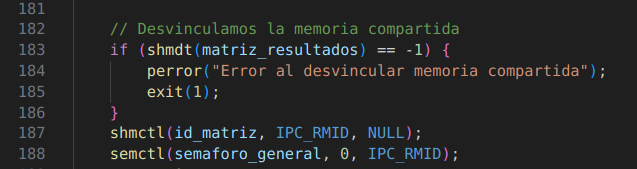
\includegraphics[width=0.9\linewidth]{Figures/codigo/cierre.png}
    \caption[Cierre del programa y liberación de recursos]{Código que muestra el cierre del programa y la liberación de recursos.}
    \label{fig:cierre-programa}
\end{figure}


\section{Análisis de la aproximación mediante serie de Fourier}

Se presenta un análisis detallado de una aproximación mediante series de Fourier para la función lineal:

\[
f(x) = 6 - 4x
\]

El análisis se apoya en una hoja de cálculo que contiene diversas columnas clave para el estudio. La columna B representa los valores de \(x\), que varían desde aproximadamente \(-3.14\) hasta \(3.01\), distribuidos en incrementos regulares que permiten observar el comportamiento de la función y su aproximación punto por punto. A continuación, las columnas que van de la C a la M están dedicadas a los términos individuales de la serie de Fourier, calculados para distintos valores de \(n\) que van desde 0 hasta 10. Cada término se obtiene usando la fórmula:

\[
\text{Término}_n = \frac{8}{n} \cdot (-1)^n \cdot \sin(n \cdot x)
\]

lo cual refleja una serie formada exclusivamente por funciones seno. Esto se debe a que la función original es impar o está definida en un intervalo simétrico.

La columna N muestra la suma de todos los términos de Fourier para cada valor de \(x\), lo que constituye la aproximación final de la serie a la función original. Esta suma se representa como:

\[
\text{Aproximación}(x) = \sum_{n=0}^{10} \text{Término}_n
\]

donde se van acumulando los valores individuales de los términos previamente calculados. Por otro lado, las columnas AA y AB proporcionan una referencia directa con la función original. En la columna AA se colocan nuevamente los valores de \(x\) utilizados, replicando los de la columna B, mientras que en la columna AB se calcula el valor exacto de la función \(f(x) = 6 - 4x\) para cada entrada, lo cual permite contrastar la aproximación de la serie con el valor real esperado.

Al observar los resultados, se encuentra que la aproximación de la serie es especialmente precisa en los puntos cercanos al origen. Por ejemplo, cuando \(x = 0.01\), el valor aproximado es \(5.9999\), muy cercano al valor exacto de 6. En contraste, para valores extremos del intervalo, como \(x = -3.14\), la diferencia entre la aproximación y el valor exacto se vuelve considerable. En este caso, la serie devuelve un valor aproximado de \(6.1274\), mientras que el valor real de la función es \(18.56\), evidenciando una discrepancia notable.

Esta diferencia creciente hacia los extremos del intervalo puede explicarse por el fenómeno de Gibbs, característico de las series de Fourier, que provoca oscilaciones cerca de discontinuidades o transiciones abruptas en funciones periódicas. A pesar de que la función analizada es lineal y continua, la representación periódica implícita en la serie introduce errores en los bordes. Además, el hecho de que solo se utilicen términos de seno confirma que se trata de una función impar o bien que ha sido definida de forma simétrica en torno al eje vertical. Finalmente, la fórmula empleada corresponde a un desarrollo típico de serie de Fourier, ampliamente utilizado en la aproximación de funciones periódicas y como herramienta fundamental en el análisis de señales y sistemas.
